% hello
\documentclass{article}

\usepackage[utf8]{inputenc}
\usepackage{graphicx}
\usepackage[dvipsnames]{xcolor}
\usepackage{csquotes}
\usepackage{hyperref}
\usepackage{tabularx}
\usepackage{booktabs}
\usepackage{pdfpages}
\usepackage{caption,geometry}
\usepackage[toc,page]{appendix}
\newcommand\myshade{85}
\colorlet{mylinkcolor}{violet}
\colorlet{mycitecolor}{YellowOrange}
\colorlet{myurlcolor}{Aquamarine}

\hypersetup{
  linkcolor  = mylinkcolor!\myshade!black,
  citecolor  = mycitecolor!\myshade!black,
  urlcolor   = myurlcolor!\myshade!black,
  colorlinks = true,
}

\usepackage[acronym]{glossaries}

\usepackage{listings}
\lstset{
    frame=Trbl,
    numbers=left,
    breaklines=true,
    basicstyle=\ttfamily,
    postbreak=\mbox{\textcolor{red}{$\hookrightarrow$}\space}
}

\usepackage[maxnames=3,style=authoryear,natbib=true]{biblatex}
\addbibresource{./references.bib}
% \bibliographystyle{unsrtnat}
% \setcitestyle{authoryear}


\newglossary[bsg]{bus}{bsd}{bsn}{Bussiness glossary}
\newglossary[dmg]{dm}{dmd}{dmn}{Data mining glossary}

\graphicspath{ {../images/} }

\DeclareUnicodeCharacter{2008}{-}% support older LaTeX versions
\DeclareUnicodeCharacter{2003}{ }% support older LaTeX versions

\let\oldautoref\autoref
\renewcommand{\autoref}[1]{(\oldautoref{#1})}
\newcommand{\autorefsub}[2]{(\oldautoref{#1}, #2)}
\newcommand{\gmt}{\acrshort{gmt}}
\newcommand{\firstvis}{first-visit data }
\newcommand{\secondvis}{second-visit data }

\newcommand{\uu}{Utrecht University}
\newcommand{\flup}{\gls{d:flup} }
\newcommand{\simon}{\gls{d:simon} }
\newcommand{\dpaper}{the \flup paper }
\newcommand{\Dpaper}{The \flup paper }
\newcommand{\spaper}{the \simon paper }

\newcommand{\MyTitle}[1]{
    \title{
    {#1}\\
    {\large Utrecht University}\\
    }
    \author{Mike Vink}
    \date{ \today }
    \maketitle
}
\newcommand{\f}[3]{%
\begin{figure}[htpb]
    \includegraphics[width=\textwidth]{#1}
    \caption{#2}
    \label{#3}
\end{figure}
}

\newcommand{\fptable}[5]{%

\newgeometry{scale=1}
\thispagestyle{empty}

\begin{table}
{%
    \centering
    \includegraphics[scale=.7]{#1}
    \captionsetup{width=0.8\linewidth}
    \captionof{table}{\textbf{#3} #4}
    \par
    \label{#5}
}
\end{table}

\restoregeometry
}

\newcommand{\fpfig}[5]{%

\newgeometry{scale=1}
\thispagestyle{empty}

\begin{figure}
{%
    \centering
    \includegraphics[scale=.7]{#1}
    \captionsetup{width=0.8\linewidth}
    \captionof{figure}{\textbf{#3} #4}
    \par
    \label{#5}
}
\end{figure}

\restoregeometry
}



\makeglossaries
\newglossaryentry{bu:rnaVirus}
{
    type=bus,
    name=ribonucleic acid virus(es),
    description={An \acrshort{rna} virus is a virus that has \acrshort{rna} as
    its genetic material. Inside a host cell this material is used to generate
    new virusses. Notable human diseases caused by RNA viruses include the
    common cold and influenza}
}
\newglossaryentry{bu:antigen}
{
    type=bus,
    name=antigen,
    description={In immunology, an antigen is a molecule or molecular
    structure, such as \acrshort{ha} and \acrshort{na}, that can be bound by an
    antigen-specific \gls{bu:antibody} or immune cell receptor.  The presence of
    antigens in the body normally triggers an immune response
    }
}
\newglossaryentry{bu:glycoprotein}
{
    type=bus,
    name=glycoprotein,
    description={Glycoproteins are molecules that comprise protein and
    carbohydrate chains. Many viruses have external glycoproteins that
    help them enter bodily cells, but can also serve to be important
    therapeutic or preventative targets}
}
\newglossaryentry{bu:mutation}
{
    type=bus,
    name=mutation,
    description={Mutation of genetic material occurs thanks to its chemical
    instability. The encoded protein molecules can have single amino acid
    (protein building block) change (minor, but still in many cases significant
    change leading to disease) or wide-range amino acid changes}
}
\newglossaryentry{bu:tiv}
{
    type=bus,
    name=TIV,
    description={
        An inactivated trivalent vaccine is a vaccine consisting of \gls{bu:antigen}ic virus particles from viruses that have been grown in culture and then killed to destroy disease producing capacity.
        In practice vaccines of three main types of influenza were used, hence trivalent
    },
    first={inactivated trivalent vaccines (TIV)}
}
\newglossaryentry{bu:antibody}
{
    type=bus,
    name=antibody,
    description={ Protein used by the immune system to identify and neutralize foreign objects such as pathogenic bacteria     and viruses.
    The antibody recognizes a unique molecule of the pathogen, called an \gls{bu:antigen}}
}
\newglossaryentry{bu:titer}
{
    type=bus,
    name=titer,
    description={
    Titer is a way of expressing concentration.
    Titer testing employs serial dilution to obtain approximate quantitative information from an analytical procedure that inherently only evaluates as positive or negative.
    The titer corresponds to the highest dilution factor that still yields a positive reading
    }
}
\newglossaryentry{bu:tcell}
{
    type=bus,
    name=T-cell,
    description={
        A T cell is a type of \gls{bu:lymphocyte}.
        T cells are one of the important white blood cells of the immune system and play a central role in the adaptive immune response, for example generating antibodies against influenza.
        Groups of specific, T cell subtypes have a variety of important functions in controlling and shaping the adaptive immune response
    }
}
\newglossaryentry{bu:lymphocyte}
{
    type=bus,
    name=lymphocyte,
    description={
        A lymphocyte is a type of white blood cell in the immune system of jawed vertebrates.
        Lymphocytes include \gls{bu:tcell}, and \gls{bu:bcell}.
        These cells work together in the adaptive immune response to generate antibodies against influenza
    }
}
\newglossaryentry{bu:cd8pos}
{
    type=bus,
    name=CD8+ T-cell,
    description={
        A cytotoxic T cell (also known as CD8+ T-cell) is a \gls{bu:tcell} that kills cancer cells, cells that are infected (particularly with viruses), or cells that are damaged in other ways.
        It does so by recognizing specific part of \gls{bu:antigen} and then starting a process that kills the targetted cell
    }
}
\newglossaryentry{bu:cd4pos}
{
    type=bus,
    name=CD4+ T-cell,
    description={
        The T helper cells, also known as CD4+ cells, "help" the activity of other immune cells by releasing \gls{bu:cytokine}s.
        These cells help to polarize the immune response into the appropriate kind depending on the nature of the immunological insult (e.g. virus vs. bacterium)
    }
}
\newglossaryentry{bu:cytokine}
{
    type=bus,
    name=cytokine,
    description={
        Cytokines are a broad and loose category of small proteins important in cell signaling that bind to receptor protein on the outside of (immune) cells to fulfill their signal function
    }
}
\newglossaryentry{bu:pbmc}
{
    type=bus,
    name=PBMC,
    description={
        A peripheral blood mononuclear cell is any peripheral blood cell having a round nucleus.
        These cells consist of \gls{bu:lymphocyte} and \gls{bu:monocyte}s
    },
    first={peripheral blood mononuclear cell (PBMC)}
}
\newglossaryentry{bu:bcell}
{
    type=bus,
    name=B-cell,
    description={
        B-cells produce antibody molecules; however, these antibodies are not secreted.
        Rather, they are presented on the outside of the cell where they serve as a part of B-cell receptors.
        When a B-cell is activated by an antigen, it proliferates and differentiates into an antibody-secreting effector cell, known as a plasmablast or plasma cell
    }
}
\newglossaryentry{bu:monocyte}
{
    type=bus,
    name=monocyte,
    description={
        Monocytes are a type of white blood cell.
        Monocytes and their macrophage and dendritic cell progeny serve three main functions in the immune system.
        These are phagocytosis, antigen presentation, and cytokine production.
        Phagocytosis is the process of uptake of microbes and particles followed by digestion and destruction of this material
    }
}
\newglossaryentry{bu:hai}
{
    type=bus,
    name=HAI,
    description={
        The \acrlong{ha} inhibition assay is used to measure the \gls{bu:titer} of \gls{bu:antibody} against a strain of influenza virus present in the serum.
        Antibody levels are measured before vaccination and 28 days after.
        The antibody levels are used to compute the seroprotection and seroconversion criteria
    },
    first={\acrlong{ha} inhibition assay (HAI)}
}
\newglossaryentry{bu:cmv}
{
    type=bus,
    name=CMV,
    description={
        Cytomegalovirus (CMV) is a common herpesvirus found in humans.
        Like other herpesviruses, it is a life-long infection that remains in a latent state inside the human body, until it is 'reactivated' by appropriate conditions.
        Thought to accelerate aging of the immune system and thereby impairing influenza vaccine response  \citep{van_den_Berg_2019}
    },
    first={cytomegalovirus (CMV)}
}
\newglossaryentry{bu:ebv}
{
    type=bus,
    name=EBV,
    description={
        The Epstein–Barr virus (EBV), is one of the nine known human herpesvirus types in the herpes family, and is one of the most common viruses in humans.
    },
    first={Epstein-Barr virus (EBV)}
}
\newglossaryentry{bu:seropc}
{
    type=bus,
    name=seroconversion and seroprotection,
    description={
        A vaccine is considered succesful if the recipient seroconverted (4-fold or greater rise in antibody against virus after vaccination) and were seroprotected (\acrshort{gmt} \(\ge\) 40) after vaccination.
    }
}
\newglossaryentry{bu:stat}
{
    type=bus,
    name=STAT,
    description={
        A vaccine is considered succesful if the recipient seroconverted (4-fold or greater rise in antibody against virus after vaccination) and were seroprotected (\acrshort{gmt} \(\ge\) 40) after vaccination.
    },
    first={signal transducers and activators of transcription (STAT)}
}



\newglossaryentry{d:model}
{
    type=dm,
    name=model,
    description={model is a model}
}
\newglossaryentry{d:flup}
{
    type=dm,
    name=FluPrint,
    description={Data used in this work}
}
\newglossaryentry{d:simon}
{
    type=dm,
    name=SIMON,
    description={Follow up study used in this work}
}

\newacronym{ha}{HA}{hemagglutinin}
\newacronym{na}{NA}{neuraminidase}
\newacronym{rna}{RNA}{ribonucleic acid}


\begin{document}
\MyTitle{Data Preparation and Modelling Report}
\tableofcontents
\printglossary[type=bus]
\printglossary[type=dm]
\printglossary[type=\acronymtype]

\section{Data selection}

The data that we use in this work is based on the data used in the simon
manuscript \citep{tomicSIMONAutomatedMachine2019}. This subset of the fluprint
database comprises data from 5 clinical studies, most importantly the
longitudal study SLVP015. It only uses the first visits of donors, as the
classification is the most complete in this dataset
\autoref{fig:dataRepeatvisits}. We will use this dataset to model the high
vaccine response with as predictors the in total 3285 features measured in
assays done by the clinical studies. The data will be prepared in the same way
as in the original work, using the mulset algorithm
\citep{tomicSIMONAutomatedMachine2019}.

\begin{figure}
    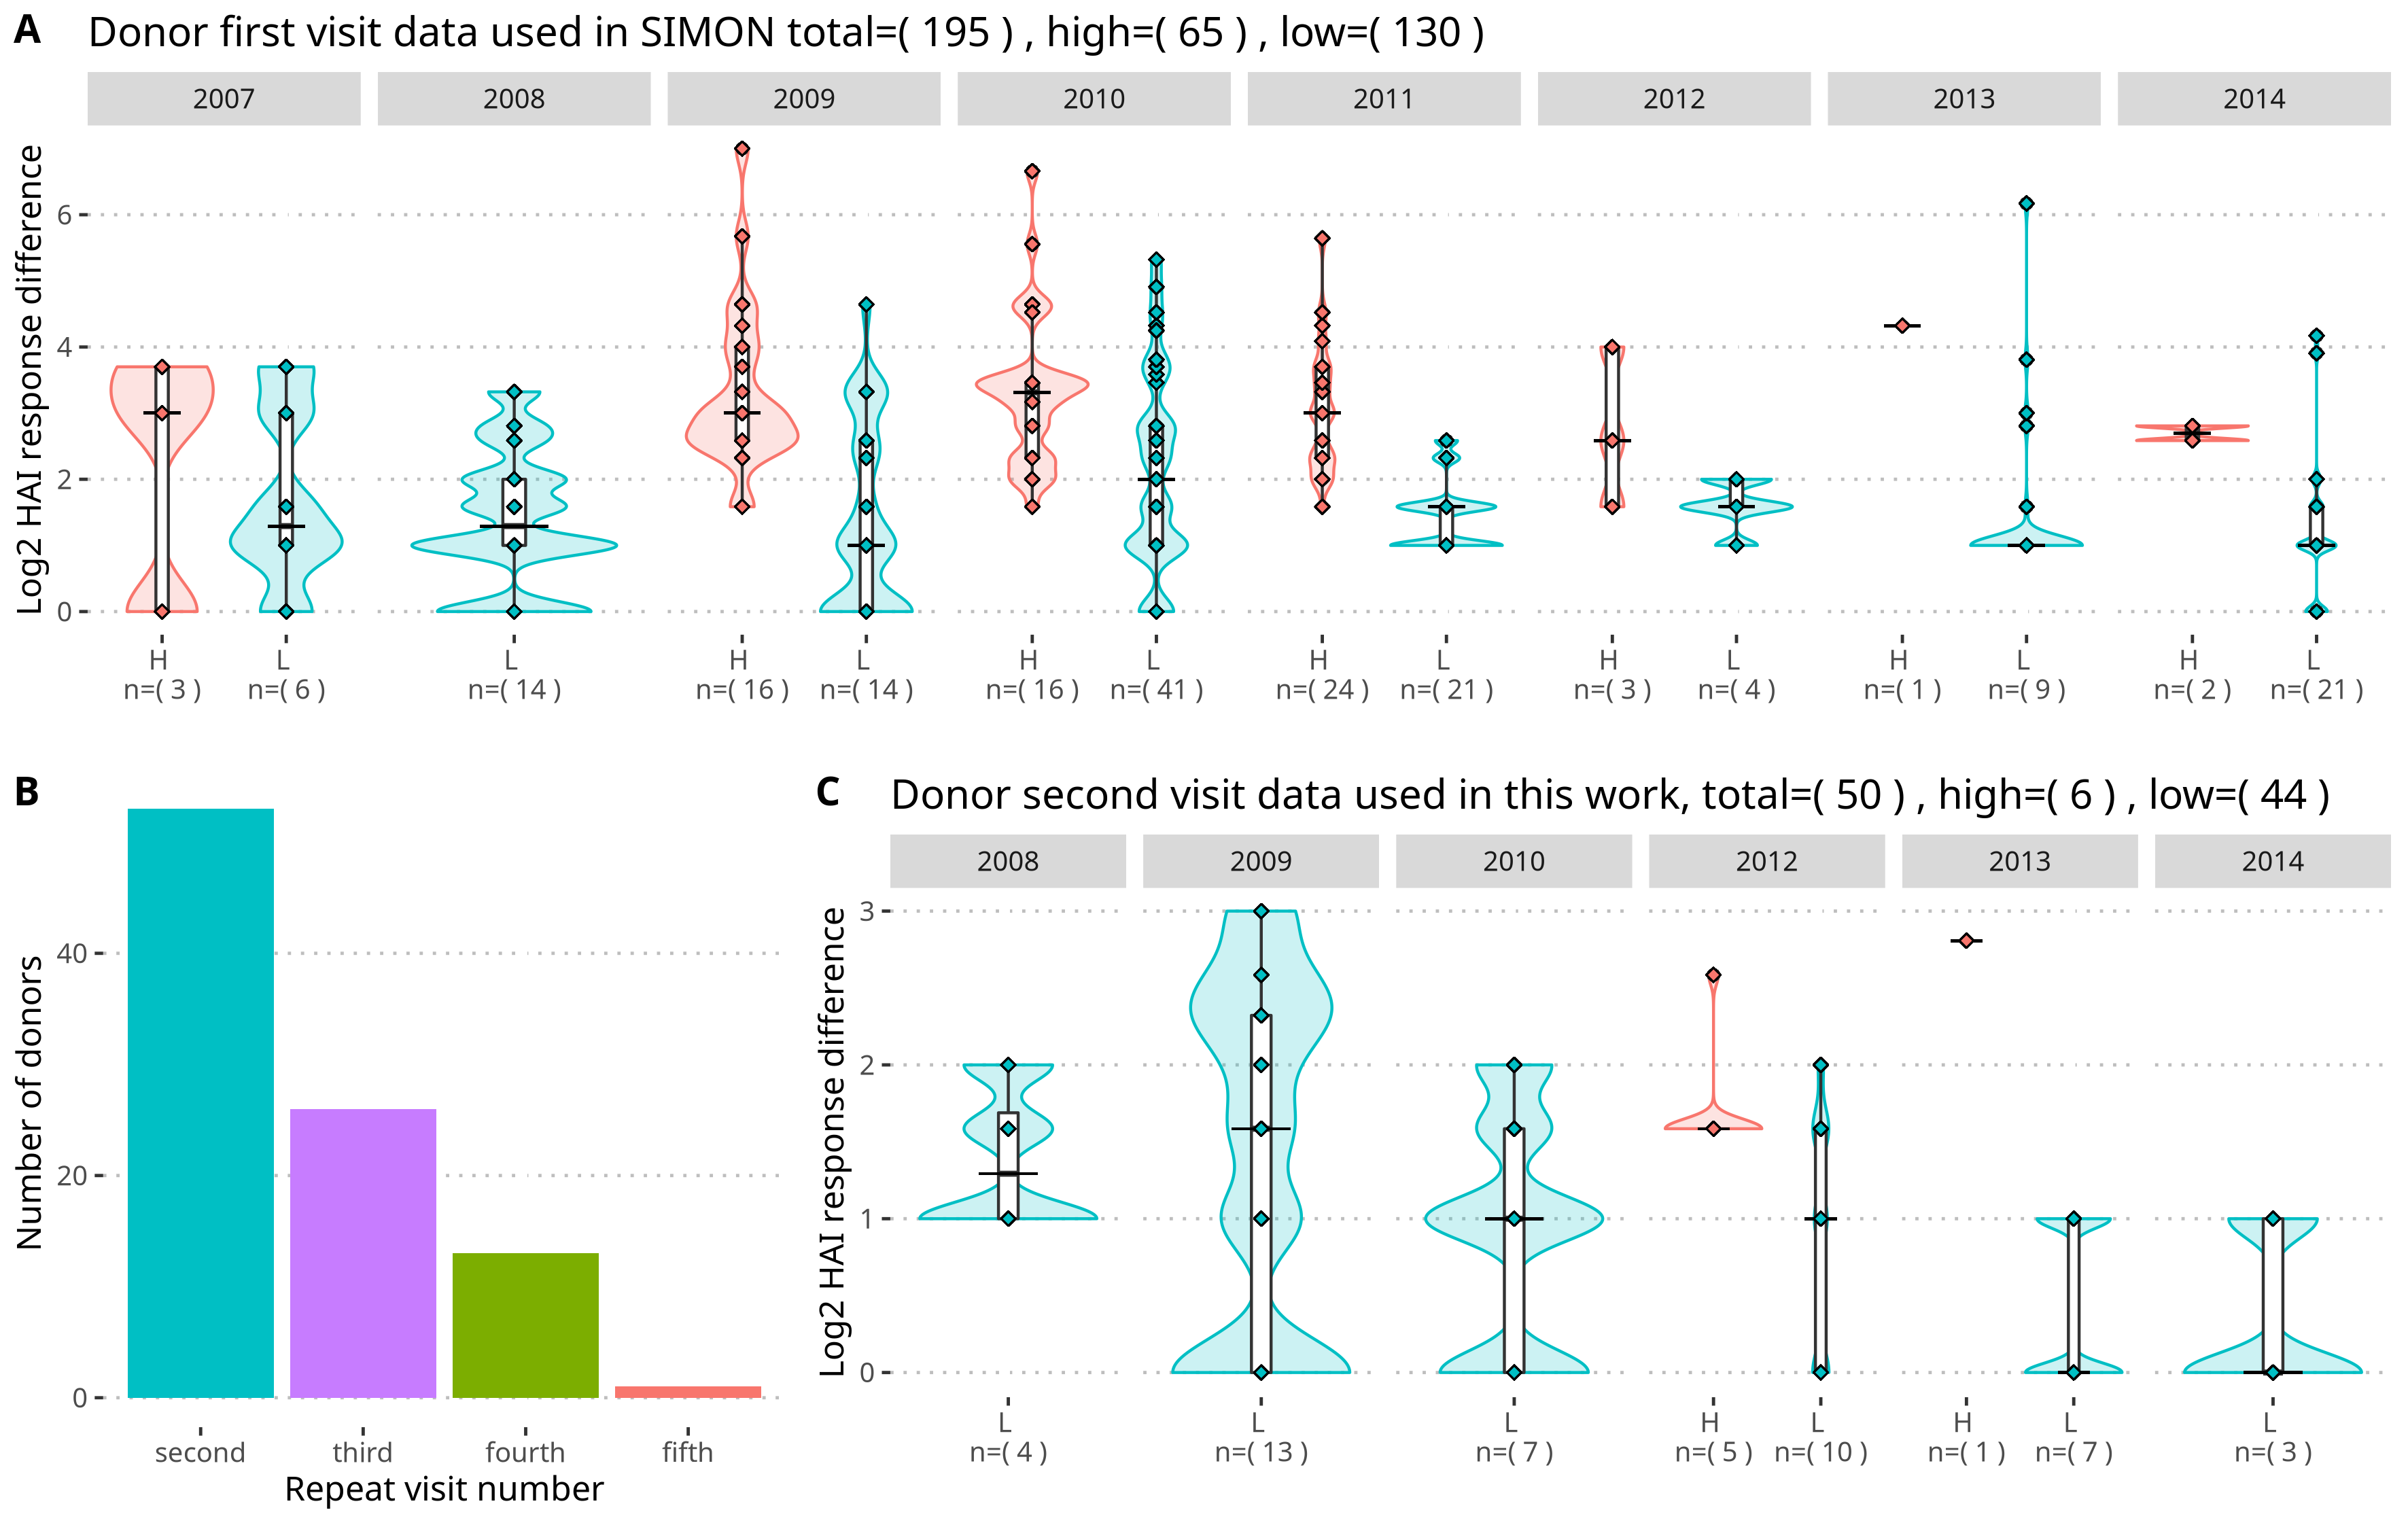
\includegraphics[width=\textwidth]{data_selection}
    \caption{caption}\label{fig:dataRepeatvisits}
\end{figure}

In addition to repeating a similar procedure as in
\cite{tomicSIMONAutomatedMachine2019}, we will compare the values of features
selected by the models trained on the first visit data to those of second visit
data. Initially the plan was to train new models on the second visit data,
however the classes are extremely unbalanced in the data of repeat visits
\autoref{fig:dataRepeatvisits}. For example in the first visit there are 65
high responders and 130 low responders, in the second visit there is only data
available for 6 high responders and 44 low responders. Therefore we will only
train model on first visit data, and use the knowledge gained to explore second
visit data.

\section{Clean data}

The goal is to obtain one or more tables from the simon data suitable to train
models, thus we are looking to change the data from the long format as in the
database in a wide format where each column is a features measured in an assay.
When attempting to do this it was discovered that some assay data contained
duplicate readouts \autoref{tbl:exampleDuplicate}. Since the values were all
similar it was decided to aggregate the values to unique features using the
mean value.

\begin{table}
\addtolength{\leftskip} {-2cm} % increase (absolute) value if needed
\addtolength{\rightskip} {-2cm} % increase (absolute) value if needed
\begin{tabular}{rrrrrlrllrrl}
\toprule{}
donor\_id & study & age & outcome & year & type & hai\_response & name & data\_name & assay & data & dup\\
\midrule{}
285 & 18 & 9.47 & 0 & 2009 & pre & 1 & CD4+ T cells & CD4\_pos\_T\_cells & 13 & 33.8 & TRUE\\
285 & 18 & 9.47 & 0 & 2009 & pre & 1 & CD4+ T cells & CD4\_pos\_T\_cells & 13 & 34.1 & TRUE\\
285 & 18 & 9.47 & 0 & 2009 & pre & 1 & CD4+ T cells & CD4\_pos\_T\_cells & 13 & 34.3 & TRUE\\
285 & 18 & 9.47 & 0 & 2009 & pre & 1 & CD4+ T cells & CD4\_pos\_T\_cells & 13 & 33.0 & TRUE\\
\bottomrule{}
\end{tabular}
    \caption{}\label{tbl:exampleDuplicate}
\end{table}

The obtained first visit wide data had dimensions of 195x3284 (donors by
measured features), with 596736 missing value cells (93\% sparsity). The second
visit data had dimensions of 50x3251, with a lower sparsity (58\%) since the donor
population is smaller and they are from the same clinical study.

\subsection{Mulset alogrithm}

Following the procedure in \cite{tomicSIMONAutomatedMachine2019} we deal with
this data sparsity by applying the mulset algorithm created by
\cite{tomicSIMONAutomatedMachine2019}. This is necessary since data is missing
in every column and the lack of prior knowledge doesn't allow for imputation of
missing values, precluding conventional measures of missing data cleaning.

\begin{figure}[ht]
    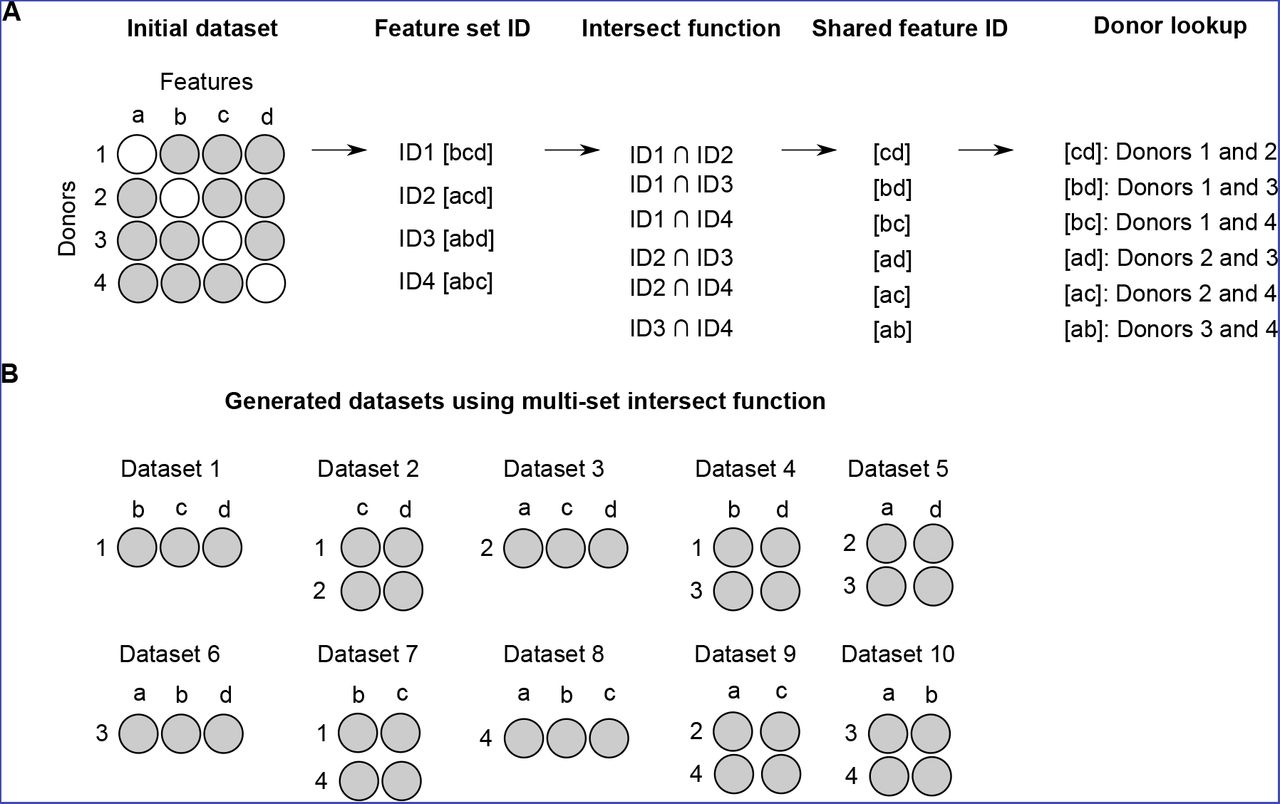
\includegraphics[width=\textwidth]{F2.large}
    \caption{\textbf{taken from original work}}\label{fig:mulsetAlg}
\end{figure}

The mulset algorithm uses the intersection of features sets of donors to
calculate pairwise shared feature sets. For every shared feature set it then
retrieves all donors that have values for these features \autoref{fig:mulsetAlg}.

\begin{lstlisting}[caption=Applying the mulset algorithm, label={lst:mulsetStep}]
% Step 1: generate re-sampled intersection datasets suitable for analysis
for {each subject in data} do:
	Calculate intersection between subject and all other subjects using mulset algorithm
	Skip sets that have less than 5 features and less than 15 donors in common
end for;
# Save all shared intersections to corresponding datasets
\end{lstlisting}

Applying the algorithm resulted in 47 different datasets without missing values
which contained a subset of donors and features, and the vaccine response
classification. Further, the same criteria as in the original work were
applied, the number of datasets was filtered down to 36 by excluding datasets
that had less than 15 donors or less than 5 features \autoref{lst:mulsetStep}.

To prepare the datasets for modelling they were partitioned into trianing and
test sets consisting of 75\% and 25\% of the data respectively. To ensure that
out of sample point estimates were not based on nonsense, datasets with a test
set containing less than 10 donors/rows were discarded. The resulting number of
cleaned datasets for modelling purposes was 20 \autoref{tbl:mulsetDatasets}. A
significant number of datasets contained more predictors than samples, however
we consider this as an inevitible phenomenon and not an absolute obstacle since
the purpose of the models is not to discriminate vaccine responders with the
highest accuracy, but to select features from that correlate with a vaccine
response from the great number of features.

\begin{table}
    \begin{tabularx}{\textwidth}{XXXXX}
\toprule{}
dataset & Rows x Cols & total (low / high (low \%)) & train (low / high) & test (low / high)\\
\midrule{}
1 & 61 x 78 & 43 / 18 ( 0.7 ) & 33 / 14 & 10 / 4\\
2 & 105 x 101 & 62 / 43 ( 0.59 ) & 47 / 33 & 15 / 10\\
3 & 140 x 50 & 94 / 46 ( 0.67 ) & 71 / 35 & 23 / 11\\
4 & 63 x 269 & 38 / 25 ( 0.6 ) & 29 / 19 & 9 / 6\\
5 & 62 x 293 & 38 / 24 ( 0.61 ) & 29 / 18 & 9 / 6\\
\addlinespace
6 & 68 x 237 & 42 / 26 ( 0.62 ) & 32 / 20 & 10 / 6\\
7 & 67 x 44 & 47 / 20 ( 0.7 ) & 36 / 15 & 11 / 5\\
8 & 111 x 93 & 66 / 45 ( 0.59 ) & 50 / 34 & 16 / 11\\
9 & 73 x 54 & 58 / 15 ( 0.79 ) & 44 / 12 & 14 / 3\\
10 & 40 x 105 & 28 / 12 ( 0.7 ) & 21 / 9 & 7 / 3\\
\addlinespace
11 & 46 x 97 & 32 / 14 ( 0.7 ) & 24 / 11 & 8 / 3\\
12 & 137 x 53 & 78 / 59 ( 0.57 ) & 59 / 45 & 19 / 14\\
13 & 48 x 42 & 35 / 13 ( 0.73 ) & 27 / 10 & 8 / 3\\
14 & 91 x 38 & 62 / 29 ( 0.68 ) & 47 / 22 & 15 / 7\\
15 & 42 x 37 & 36 / 6 ( 0.86 ) & 27 / 5 & 9 / 1\\
\addlinespace
16 & 92 x 26 & 62 / 30 ( 0.67 ) & 47 / 23 & 15 / 7\\
17 & 88 x 6 & 68 / 20 ( 0.77 ) & 51 / 15 & 17 / 5\\
18 & 82 x 87 & 56 / 26 ( 0.68 ) & 42 / 20 & 14 / 6\\
19 & 151 x 51 & 92 / 59 ( 0.61 ) & 69 / 45 & 23 / 14\\
20 & 83 x 75 & 56 / 27 ( 0.67 ) & 42 / 21 & 14 / 6\\
\bottomrule{}
\end{tabularx}
    \caption{caption}\label{tbl:mulsetDatasets}
\end{table}


\section{Modelling}

The modelling techniques of choice were to be resistent to the "too many
features" problem and suitable for selecting features in an embedded based
approach \citep{hiraReviewFeatureSelection2015}. Technically, the approach used
here is a wrapper approach since we are using the mulset algorithm to generate
different subsets of features and training machine learning models on those
features. However, in this work we train three models that have an embedded
mechanism for obtaining the most important predictors of vaccine response. This
is done for every feature set, and manually we chose the best and most
interesting trained models and their obtained features. The end goal was to
identify important features and investigating the change in those features for the
second visit/influenza season of donors.

\begin{table}
\addtolength{\leftskip} {-2cm} % increase (absolute) value if needed
\addtolength{\rightskip} {-2cm} % increase (absolute) value if needed
\begin{tabular}{llrrrrrrrrrrrrr}
\toprule{}
dataset &model & SENS & SPEC & MCC & PREC & NPV & FPR & F1 & TP & FP & TN & FN & train AUC & test AUC\\
\midrule{}
14    & rrlda & 0.091 & 0.915 & 0.010 & 0.333 & 0.683 & 0.085 & 0.143 & 2 & 4 & 43 & 20 & 0.50 & 0.62\\
    & nb & 0.636 & 0.702 & 0.321 & 0.500 & 0.805 & 0.298 & 0.560 & 14 & 14 & 33 & 8 & 0.67 & 0.59\\
    & rf & 0.364 & 0.851 & 0.243 & 0.533 & 0.741 & 0.149 & 0.432 & 8 & 7 & 40 & 14 & 0.65 & 0.61\\
    & reglog & 0.227 & 0.766 & -0.007 & 0.312 & 0.679 & 0.234 & 0.263 & 5 & 11 & 36 & 17 & 0.49 & 0.48\\
\addlinespace
16    & rrlda & 0.000 & 1.000 & NaN & NaN & 0.671 & 0.000 & 0.000 & 0 & 0 & 47 & 23 & 0.48 & 0.61\\
    & nb & 0.652 & 0.617 & 0.253 & 0.455 & 0.784 & 0.383 & 0.536 & 15 & 18 & 29 & 8 & 0.68 & 0.55\\
    & rf & 0.261 & 0.851 & 0.135 & 0.462 & 0.702 & 0.149 & 0.333 & 6 & 7 & 40 & 17 & 0.65 & 0.69\\
    & reglog & 0.391 & 0.723 & 0.116 & 0.409 & 0.708 & 0.277 & 0.400 & 9 & 13 & 34 & 14 & 0.64 & 0.47\\
\addlinespace
19    & rrlda & 0.533 & 0.391 & -0.075 & 0.364 & 0.562 & 0.609 & 0.432 & 24 & 42 & 27 & 21 & 0.47 & 0.41\\
    & nb & 0.489 & 0.565 & 0.053 & 0.423 & 0.629 & 0.435 & 0.454 & 22 & 30 & 39 & 23 & 0.54 & 0.48\\
    & rf & 0.244 & 0.739 & -0.018 & 0.379 & 0.600 & 0.261 & 0.297 & 11 & 18 & 51 & 34 & 0.54 & 0.52\\
    & reglog & 0.267 & 0.754 & 0.023 & 0.414 & 0.612 & 0.246 & 0.324 & 12 & 17 & 52 & 33 & 0.51 & 0.32\\
\bottomrule{}
\end{tabular}

\end{table}

\begin{figure}[htpb]
    \centering
    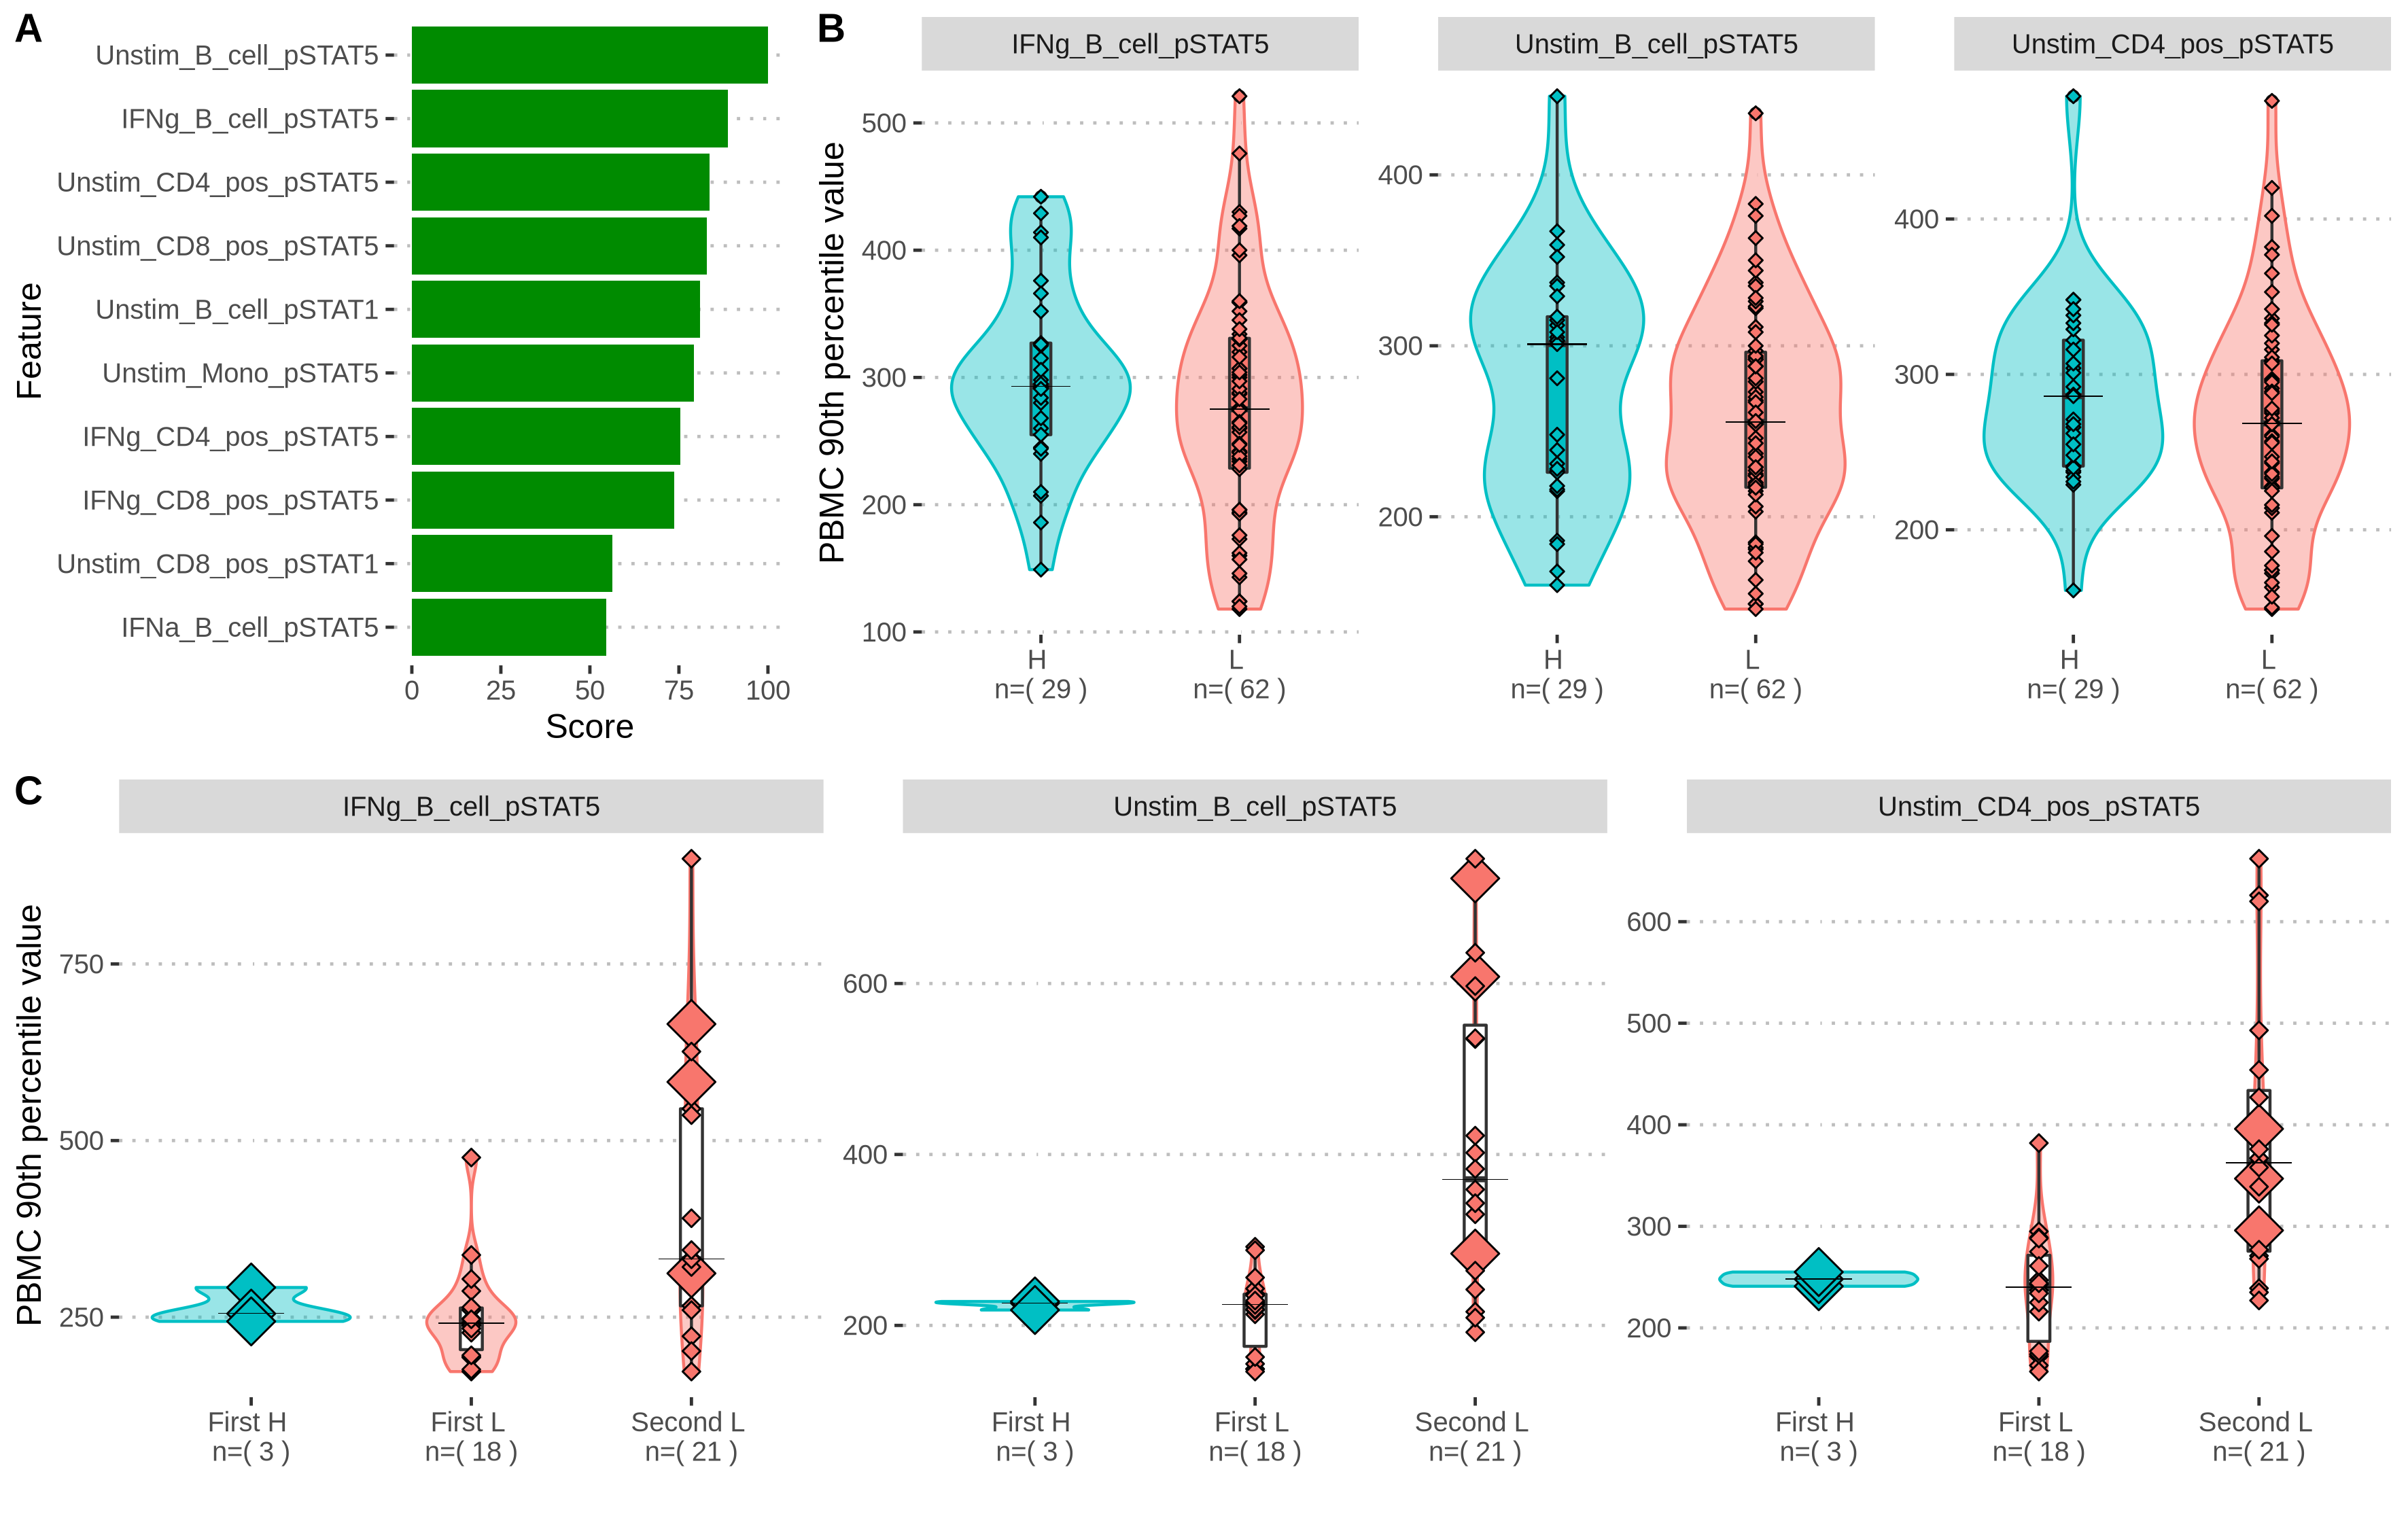
\includegraphics[width=\textwidth]{dataset1_nb_feature_exploration}
    \caption{dataset1-nb-feature-exploration}
    \label{fig:dataset1-nb-feature-exploration}
\end{figure}

\begin{figure}[htpb]
    \centering
    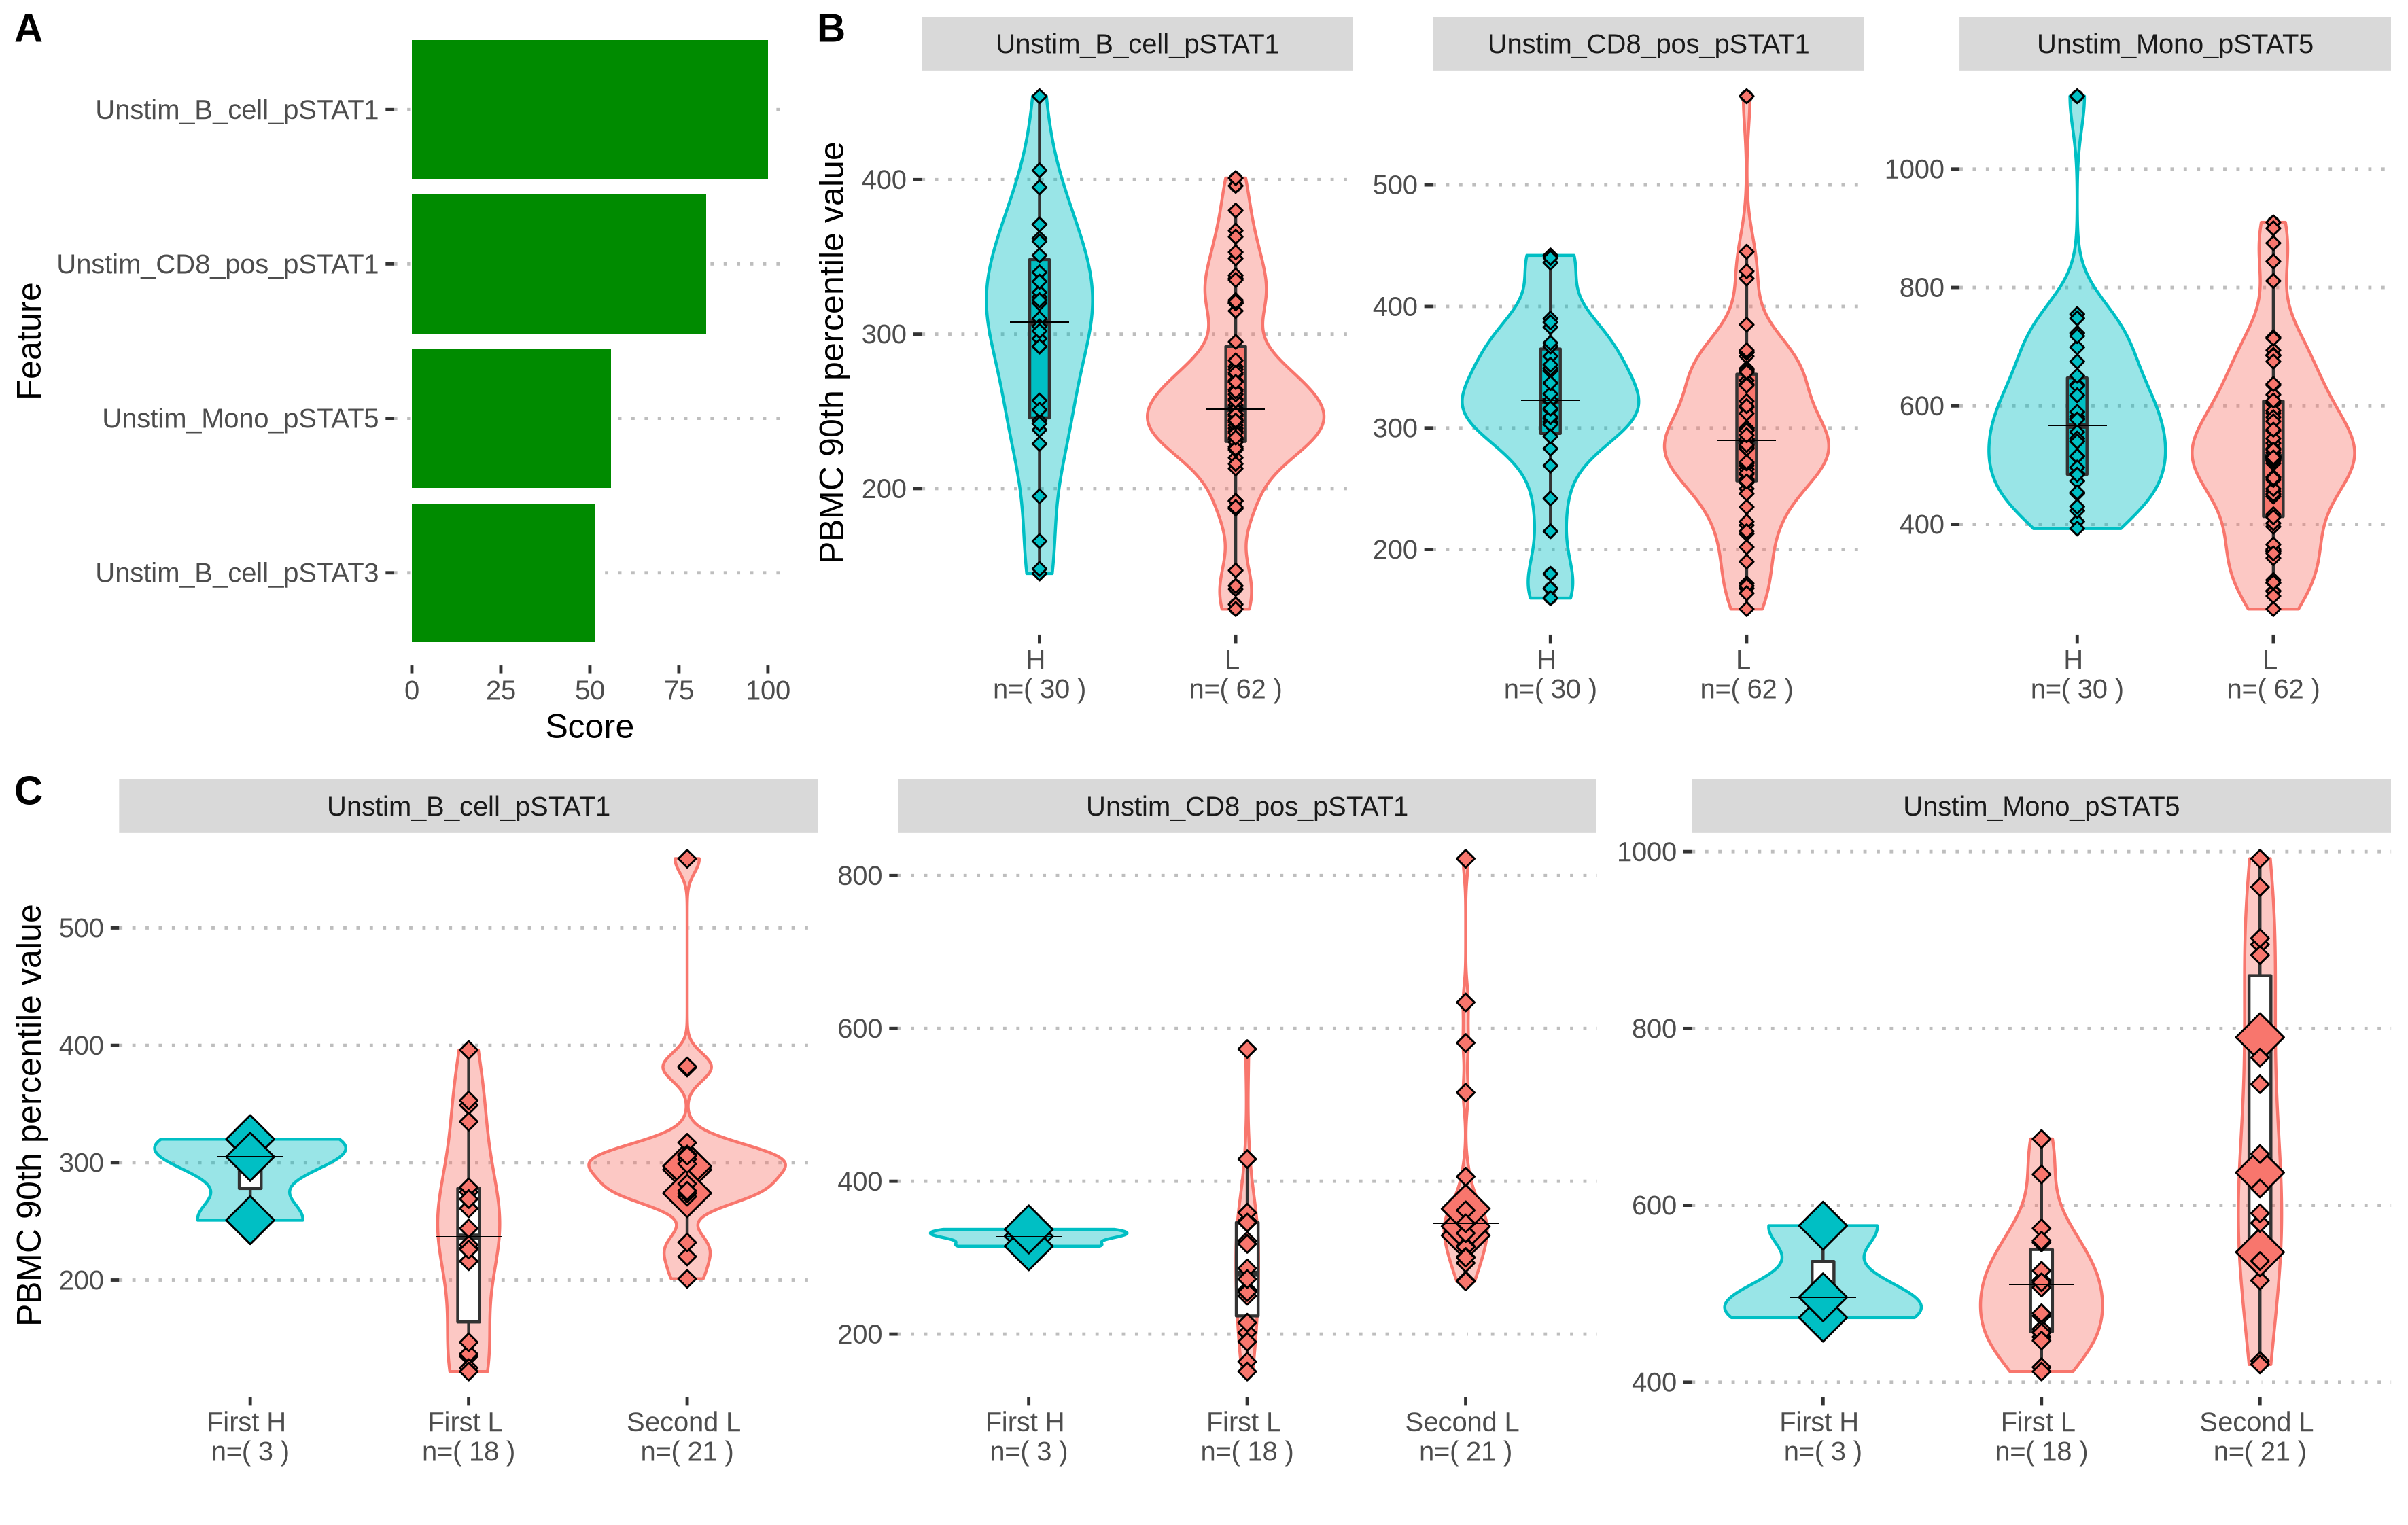
\includegraphics[width=\textwidth]{dataset2_nb_feature_exploration}
    \caption{dataset2-nb-feature-exploration}
    \label{fig:dataset2-nb-feature-exploration}
\end{figure}

\begin{figure}[htpb]
    \centering
    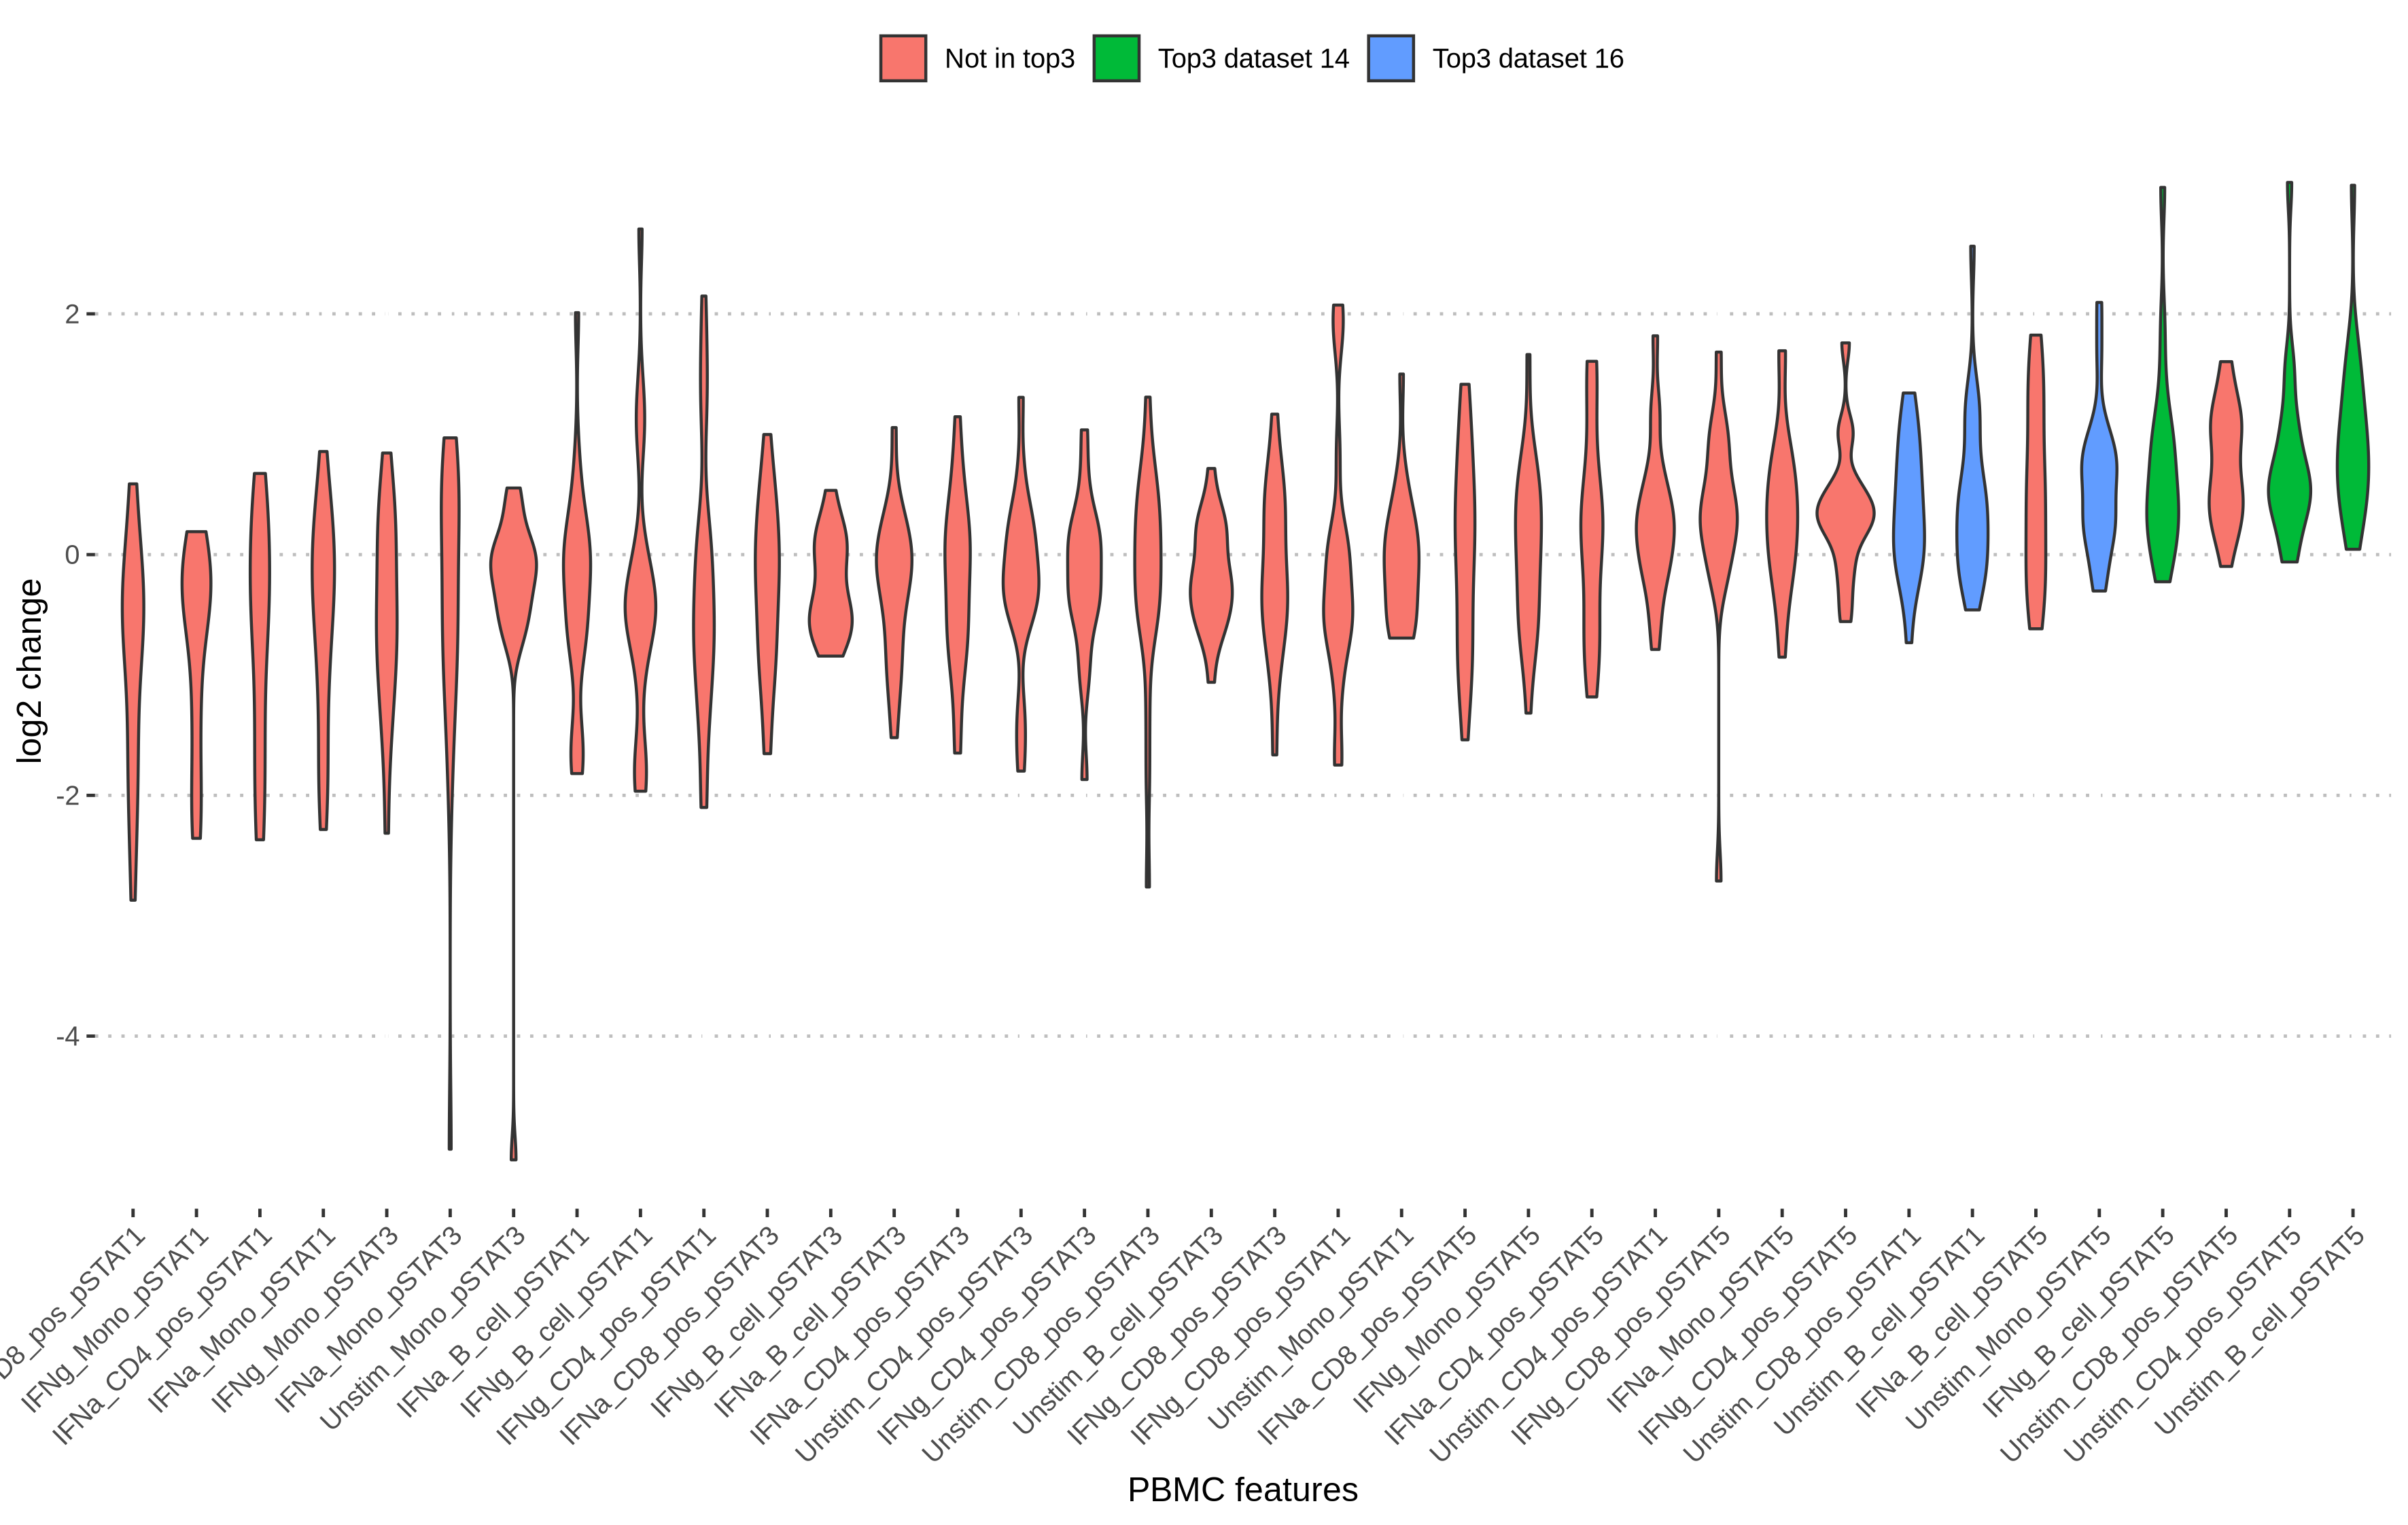
\includegraphics[width=\textwidth]{second_visit_change1}
    \caption{second-visit-change1}
    \label{fig:second-visit-change1}
\end{figure}

\begin{figure}[htpb]
    \centering
    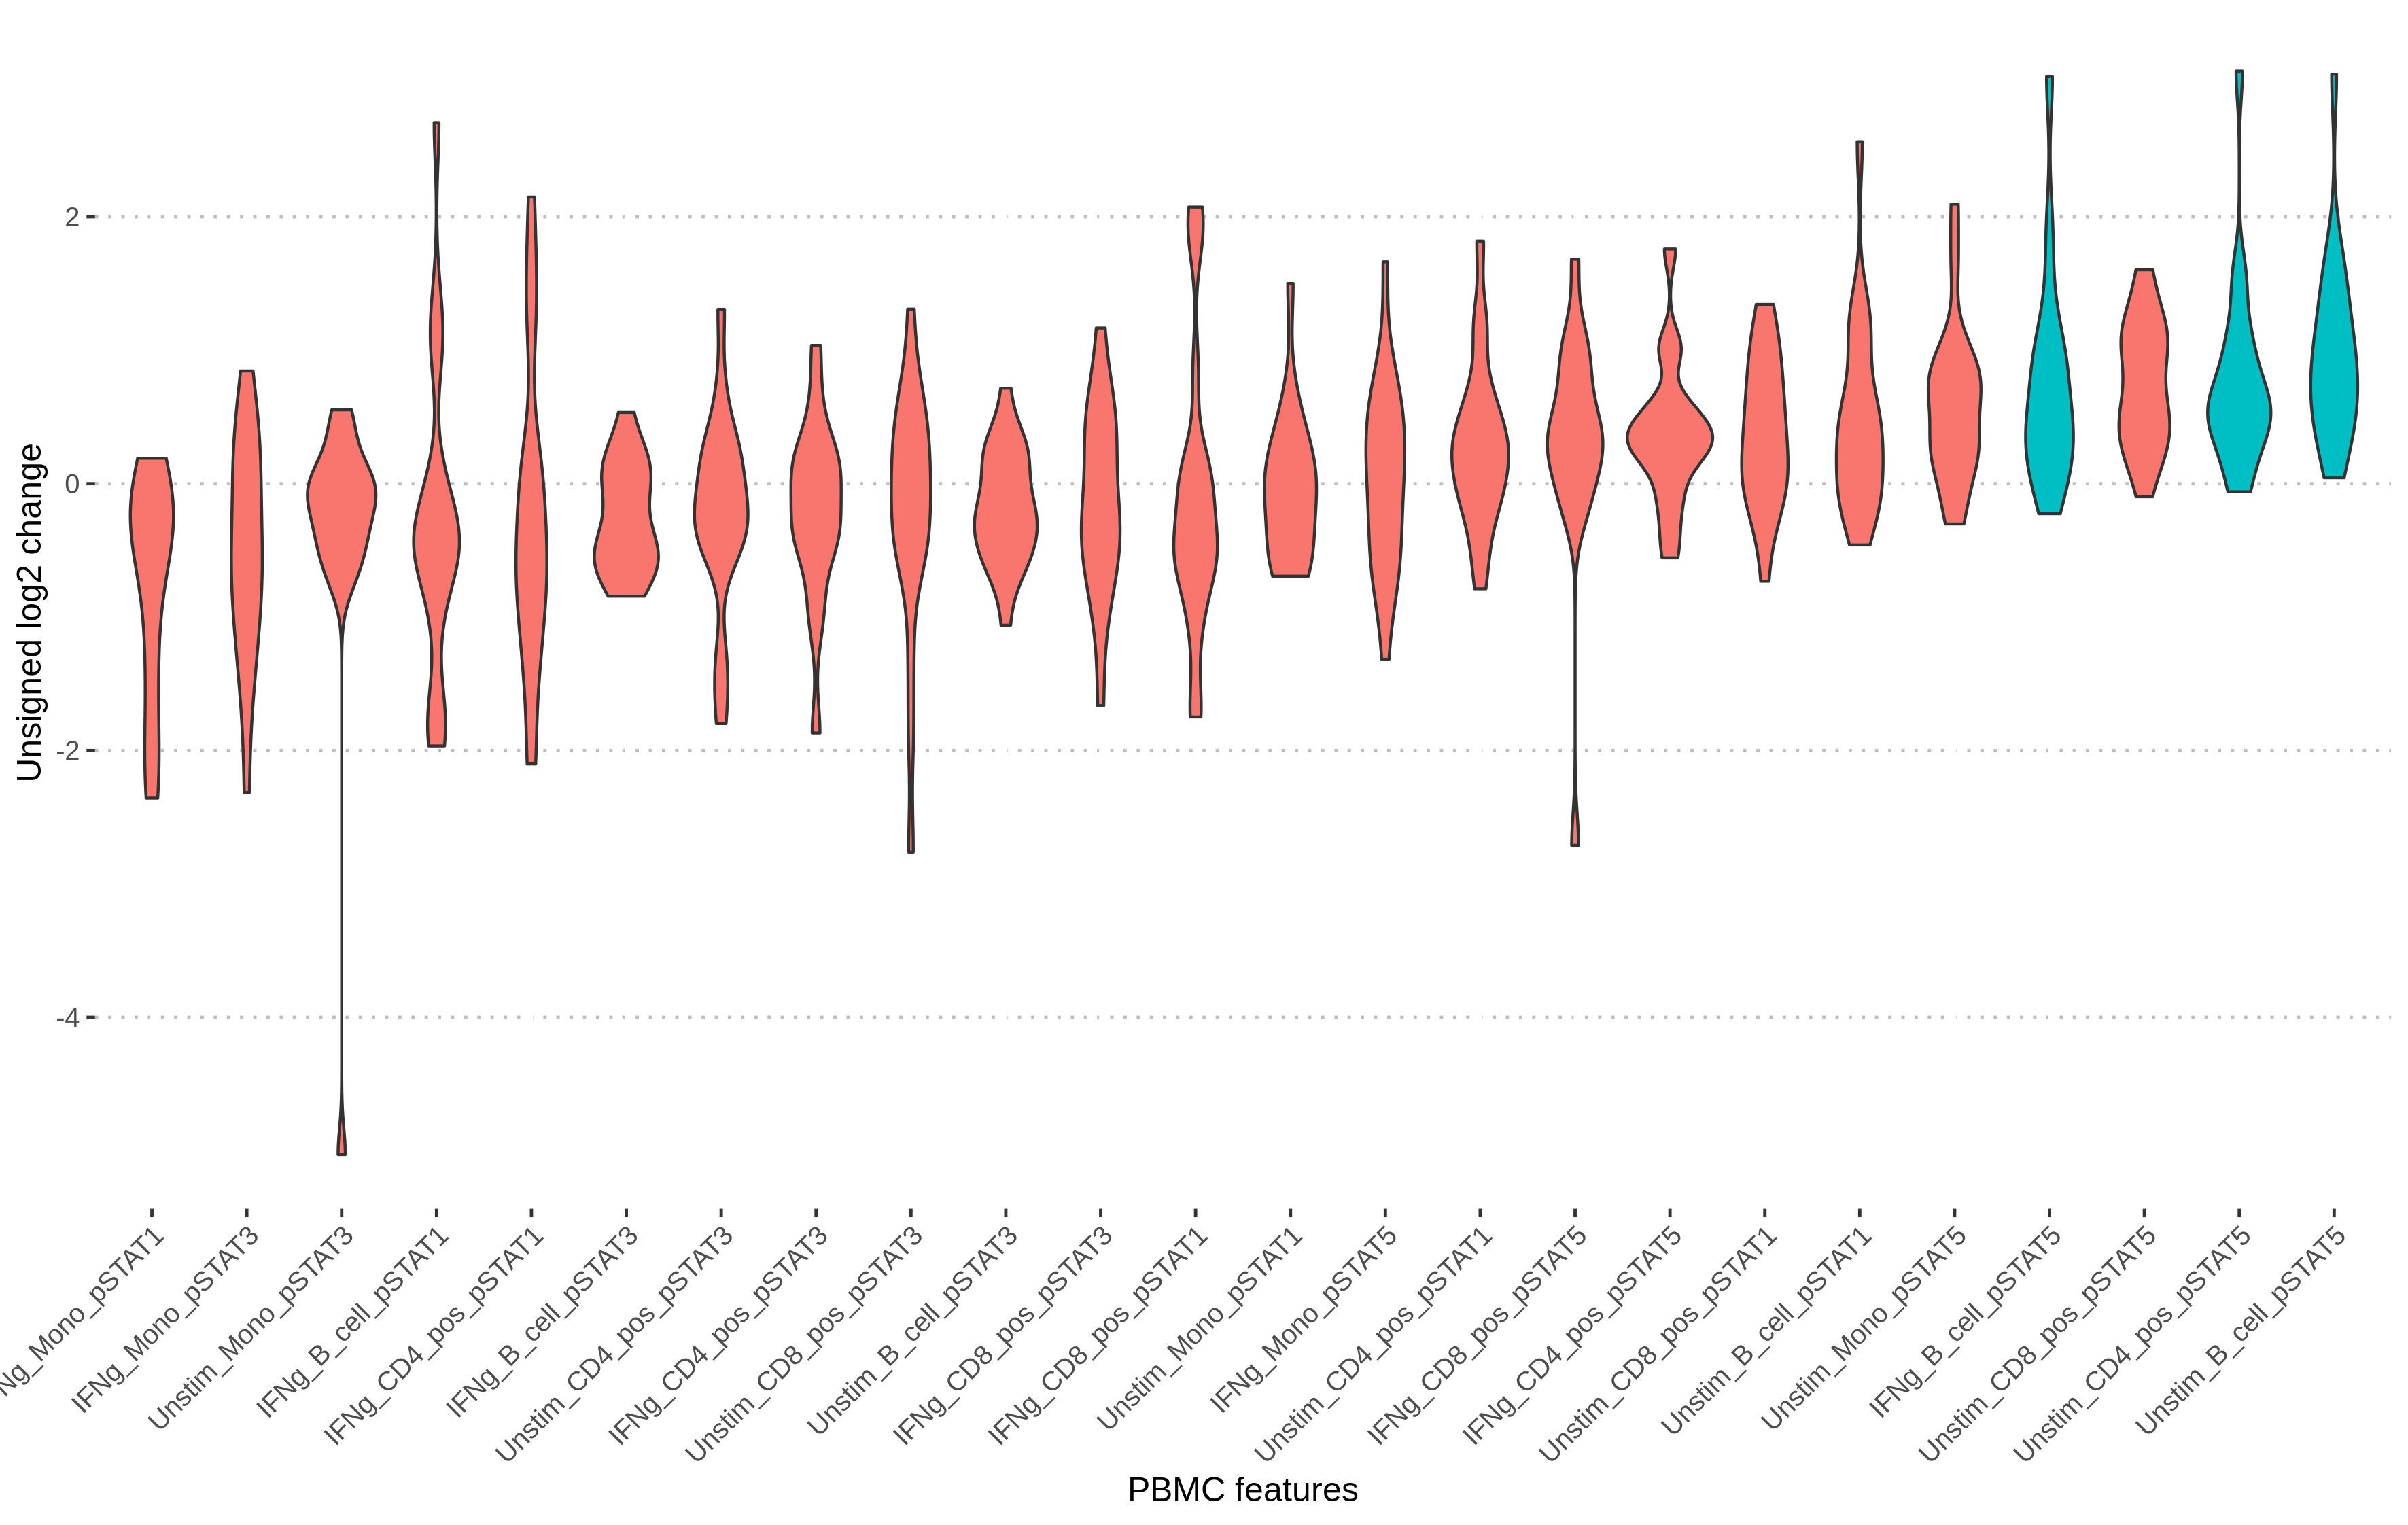
\includegraphics[width=\textwidth]{second_visit_change2}
    \caption{second-visit-change1}
    \label{fig:second-visit-change1}
\end{figure}

\begin{figure}[htpb]
    \centering
    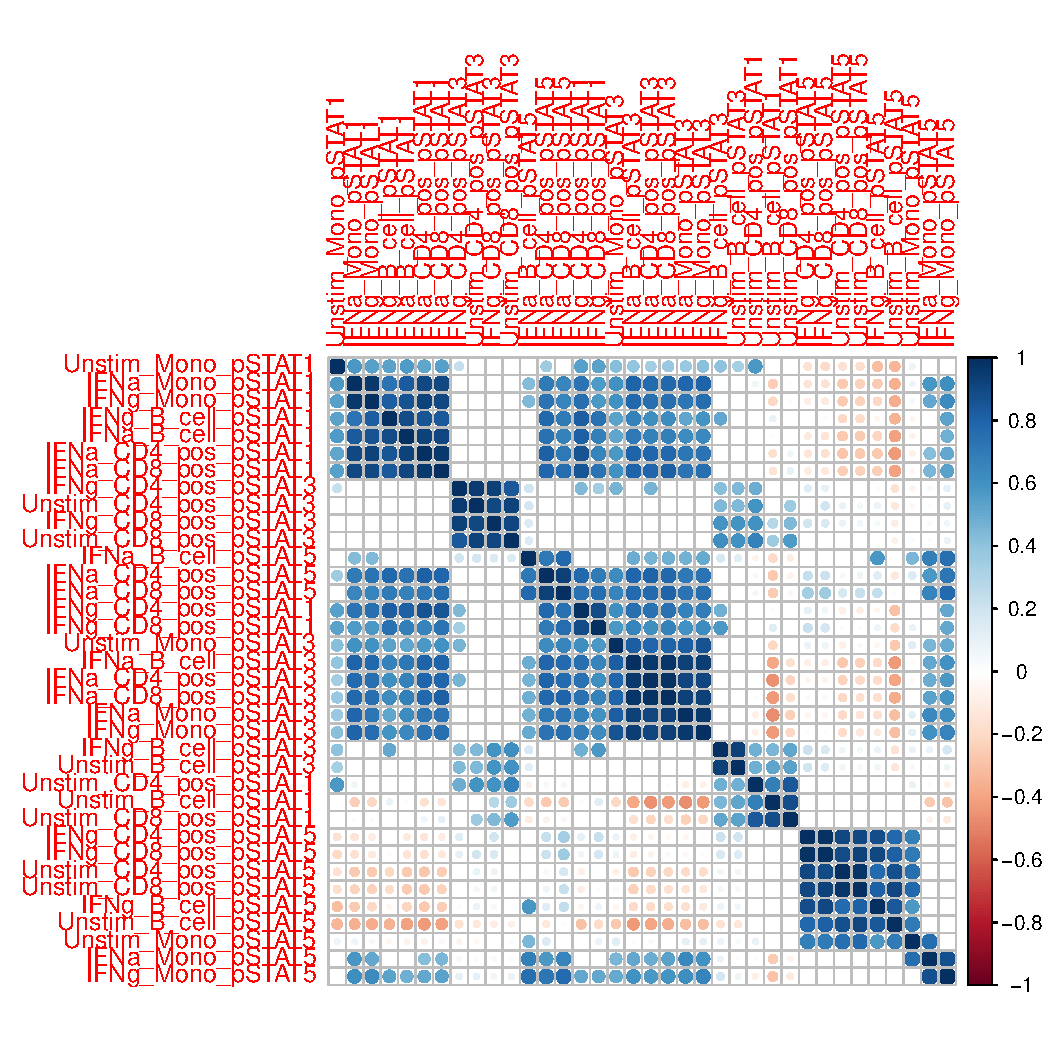
\includegraphics[width=\textwidth]{cor_dataset1}
    \caption{cor-dataset1}
    \label{fig:cor-dataset1}
\end{figure}

\begin{figure}[htpb]
    \centering
    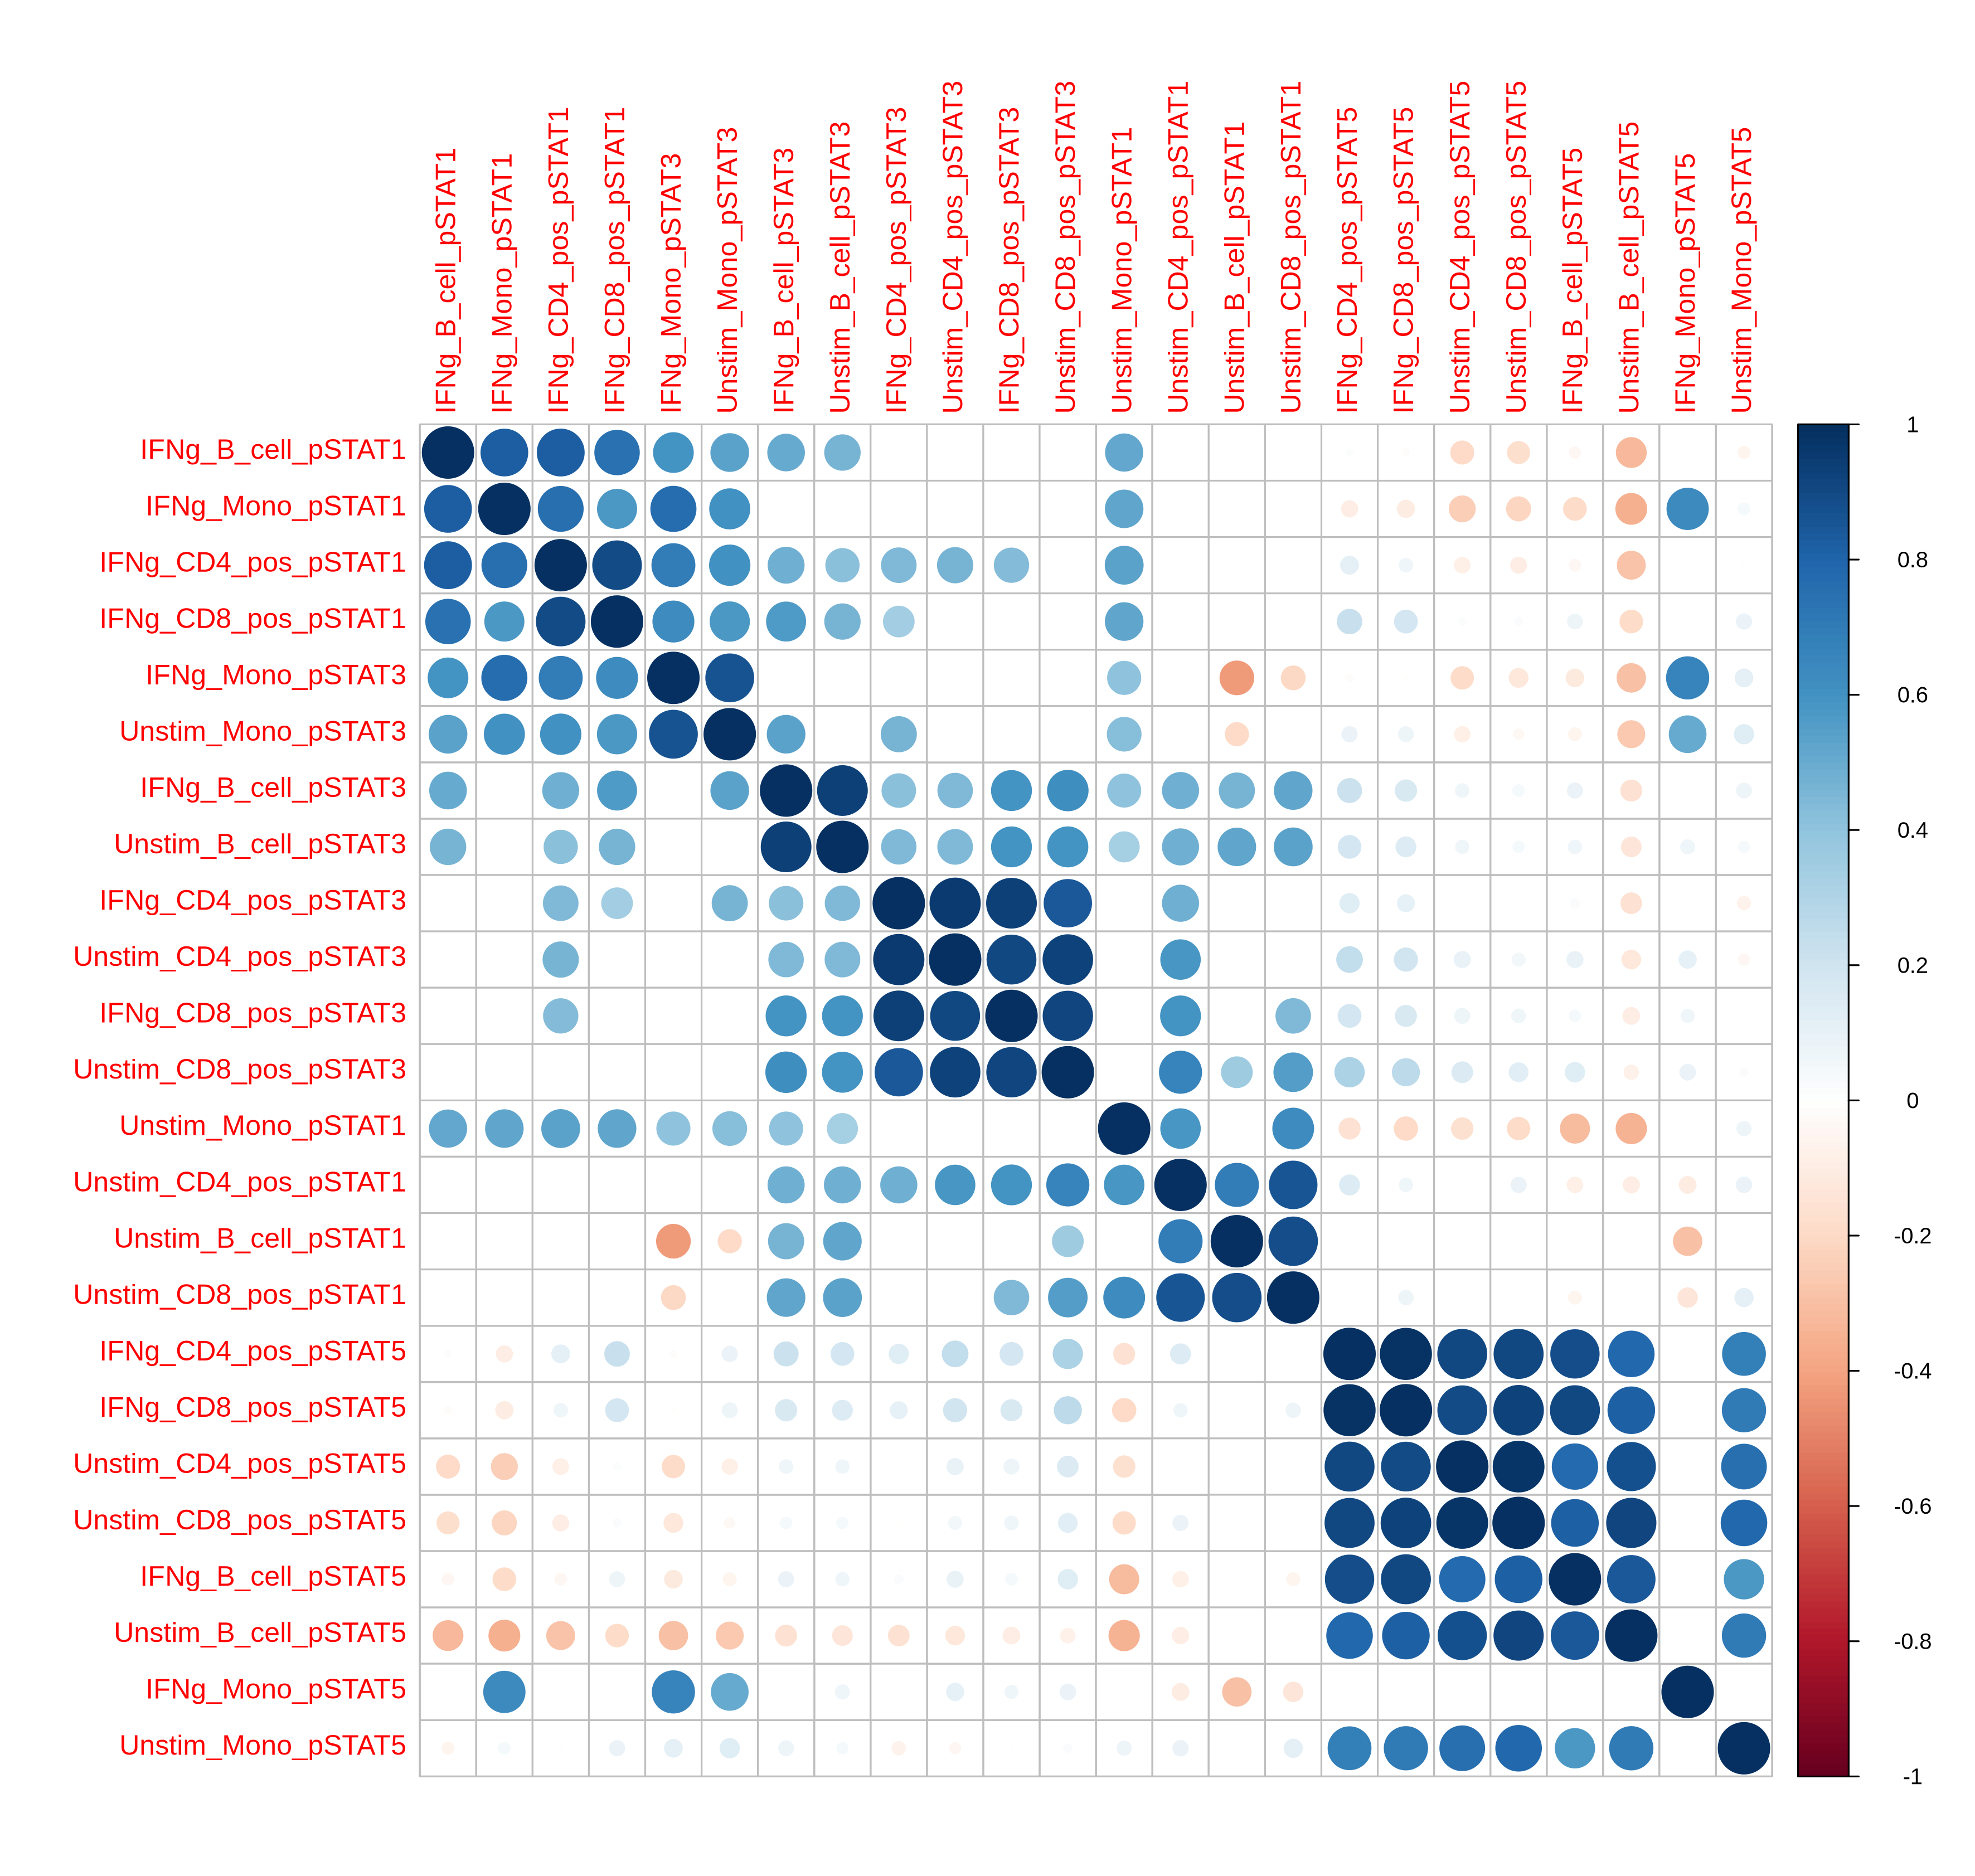
\includegraphics[width=\textwidth]{cor_dataset2}
    \caption{cor-dataset2}
    \label{fig:cor-dataset2}
\end{figure}


\end{document}
